\section{Symmetric Groups, Cycle \& Cycle Structure}
\begin{definition}
    Let $\Omega$ be any nonempty set and let $S_\Omega$ be the set of all bijections from $\Omega$ to itself. Then $S_{\Omega}$ forms a group under function composition: $\circ$. $(S, \circ)$ is called \textit{symmetric group} on the set $\Omega$.
\end{definition}
When $\Omega = \{1, 2, ..., n\}$, we write it as $S_n$. 
\begin{eg}
    Let $\Omega = \{a, b\}$.
    \[
S_\Omega = 
    \left\{
    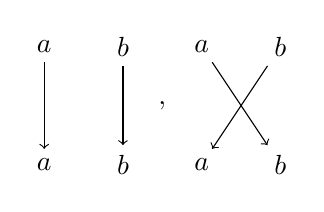
\begin{tikzpicture}[baseline={(current bounding box.center)}]
        % First mapping
        \node (a) at (0,0) {$a$};
        \node (b) at (1,0) {$b$};
        \node (a1) at (0,-1.5) {$a$};
        \node (b1) at (1,-1.5) {$b$};
        \draw[->] (a) -- (a1);
        \draw[->] (b) -- (b1);

        \node (c) at (1.5, -0.75) {$,$};
        % Second mapping
        \node (a) at (2,0) {$a$};
        \node (b) at (3,0) {$b$};
        \node (a1) at (2,-1.5) {$a$};
        \node (b1) at (3,-1.5) {$b$};
        \draw[->] (a) -- (b1);
        \draw[->] (b) -- (a1);
    \end{tikzpicture}
    \right\}
    \]
    $|S_\Omega| = 2.$
\end{eg}
\begin{eg}
    If $\Omega = \{a, b, c\}$, $|S_\Omega| = 6.$
\end{eg}
Order of $S_n$ is $n!$. Let $\sigma \in S_n$, then\\
$\sigma(1)$ has $n$ choices to send $1$ to any $n$ element.\\
$\sigma(2)$ has $(n-1)$ choices.\\
$\sigma(3)$ has $(n-2)$ choices.\\
.\\
.\\
.\\
$\sigma(n)$ has $(1)$ choices.\\
Hence, there is precisely $n(n-1)(n-2)\cdots2\cdot1 = n!$ bijections from $n$ to itself.\\
\begin{definition}
    A \textit{cycle} is a string of integers which represents the element of $S_n$ which cyclically permutes these integers (and fixes all other integers). 
\end{definition}
Let \[\sigma = \begin{pmatrix}
    1 & \rightarrow & 2\\
    2 & \rightarrow & 3\\
    3 & \rightarrow & 1
\end{pmatrix} \in S_3.\]
$\sigma^3 = e$. $\sigma$ is called cycle of length $|\sigma| = 3$ generated by $\sigma$.\\
Again, let $\sigma \in S_5$ and $\sigma$ acts as follows:
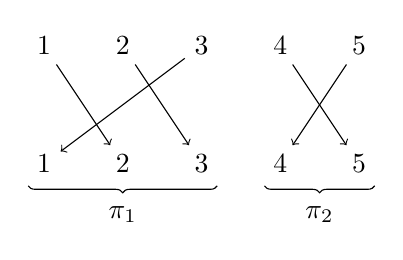
\begin{tikzpicture}[baseline={(current bounding box.center)}]
    % First mapping
    \node (a) at (0,0) {$1$};
    \node (b) at (1,0) {$2$};
    \node (c) at (2,0) {$3$};
    \node (d) at (3,0) {$4$};
    \node (e) at (4,0) {$5$};
    \node (a1) at (0,-1.5) {$1$};
    \node (b1) at (1,-1.5) {$2$};
    \node (c1) at (2,-1.5) {$3$};
    \node (d1) at (3,-1.5) {$4$};
    \node (e1) at (4,-1.5) {$5$};

    % Arrows
    \draw[->] (a) -- (b1);
    \draw[->] (b) -- (c1);
    \draw[->] (c) -- (a1);
    \draw[->] (d) -- (e1);
    \draw[->] (e) -- (d1);

    % Brackets and labels
    \draw[decorate,decoration={brace,mirror,raise=-12pt}] (-0.2,-2.2) -- (2.2,-2.2) node[midway,below=-8pt] {$\pi_1$};
    \draw[decorate,decoration={brace,mirror,raise=-12pt}] (2.8,-2.2) -- (4.2,-2.2) node[midway,below=-8pt] {$\pi_2$};
\end{tikzpicture}\\
$\sigma = \pi_1 \circ \pi_2$, where $\pi_1$ has the cycle structure $(3+1+1)$ and $\pi_2$ has the cycle structure $(2+1+1+1)$.\\
Two cycles are called \textit{disjoint} if they have no elements in common. $\pi_1, \pi_2$ are examples of disjoint cycles. Notice, \textit{two dijoint cycles commutes} as we can see they do not interact with each other.
\begin{theorem}
    Every elements in $S_n$ can be written as composition of disjoint cycles.
\end{theorem}
